\section{Observations}
\label{sec:observations}

In working in unit cube space, we encountered questions and peculiarities that we cannot fully explore in the scope of this work.  
Here we present briefly a few of the things we noticed.

The projection of a trace into cube space is sensitive to the original rotation of the chosen axes.
So far, we have chosen real-world situations where the axes are aligned with our cube space, like in our examples with flying robots, where the co-ordinates of the motion capture system and the trajectories we programmed are axes aligned.
This would not necessarily need to be the case.
We suspect that box trace properties and cube ratios will change in proportion to the rotation angle, until a maximum divergence is reached $45^{\circ}$s from the original axes.
Further rotation from $45-90^{\circ}$s will decrease divergence until a rotational symmetry is found perpendicular to the original axes.
This might mean that there are a number of `best orientations' for the cube space relative the spatial trace, and that initially searching the space of possible orientations would find a better fit from which to find properties.

\begin{wrapfigure}{l}{0.62\textwidth}
  \centering
  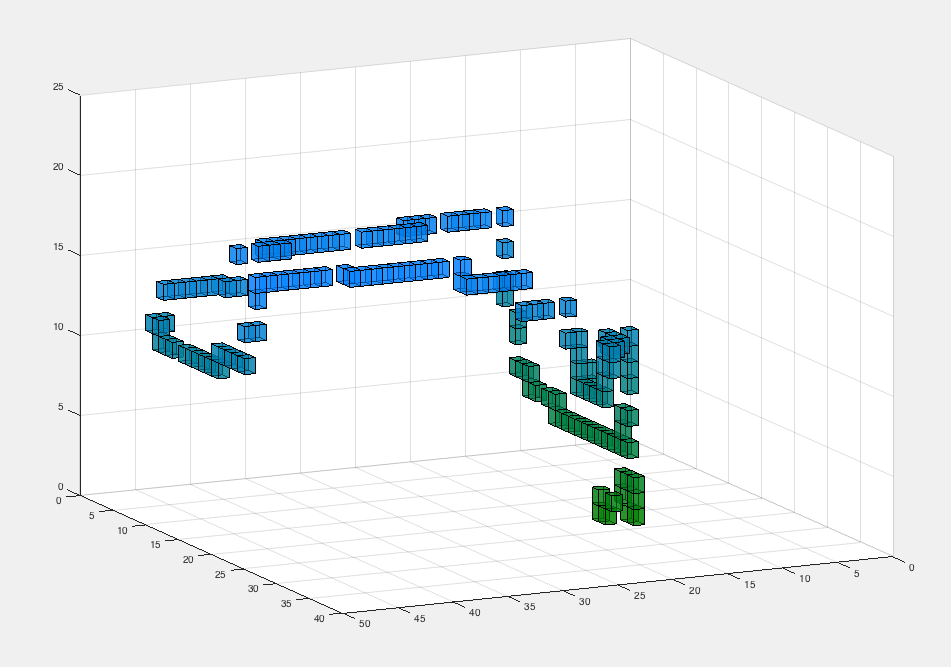
\includegraphics[width=0.62\textwidth]{./figures/cubesTooSmall.png}
  \caption{Example of $10cm$ cubes where $\phi_{teleports}$ is true}
  \label{fig:teleport}
\end{wrapfigure}

Another consideration is choosing a good cube size.  
Different sizes may generate very different properties.
If you choose \emph{too small of a cube}, the trace may model $\phi_{\{teleport\}}$, as shown in Fig.~\ref{fig:teleport}, which we define as a spatially disconnected cube-trace.
If there are gaps of disconnected cubes, and two entities collide in the unaccounted for space, the violation of cube-independence will not be inferred.
 If you choose \emph{too big of a cube}, this may be too rough of an over approximation.
For an extreme example, an entity never registers ``leaving home" if its initial cube is the size of the given dimensions.
Sometimes large over-approximations are desired, such as if you only want to examine the movements across two ``hemispheres" of an entity's space.

We are curious about moments when trajectories loiter and meander slightly near the intersection of eight cubes.
These are literally `corner cases' where several or even many nodes would be added in the graph even though the movements are very small.
It might be worth building in thresholds to ensure a spatial trace has `really' moved to the next cube.



